\chapter{Additional Figures}
\label{chapter:add-figs}

%This is the first appendix. You could put some test images or verbose data in an
%appendix, if there is too much data to fit in the actual text nicely.
%
%For now, the Aalto logo variants are shown in Figure~\ref{fig:aaltologo}.

%\begin{figure}
%\begin{center}
%\subfloat[In English]{
\includegraphics[width=.8\textwidth]{images/aalto-logo-en}}
%\subfloat[Suomeksi]{
\includegraphics[width=.8\textwidth]{images/aalto-logo-fi}}
%\subfloat[P� svenska]{
\includegraphics[width=.8\textwidth]{images/aalto-logo-se}}
%\caption{Aalto logo variants}
%\label{fig:aaltologo}
%
%\end{center}
%\end{figure}

\section{Case Studies}

\section{Deterministic Metrics}

\begin{figure}[ht]
	\label{fig:csi}
	\subfloat[0.5 mm/h]{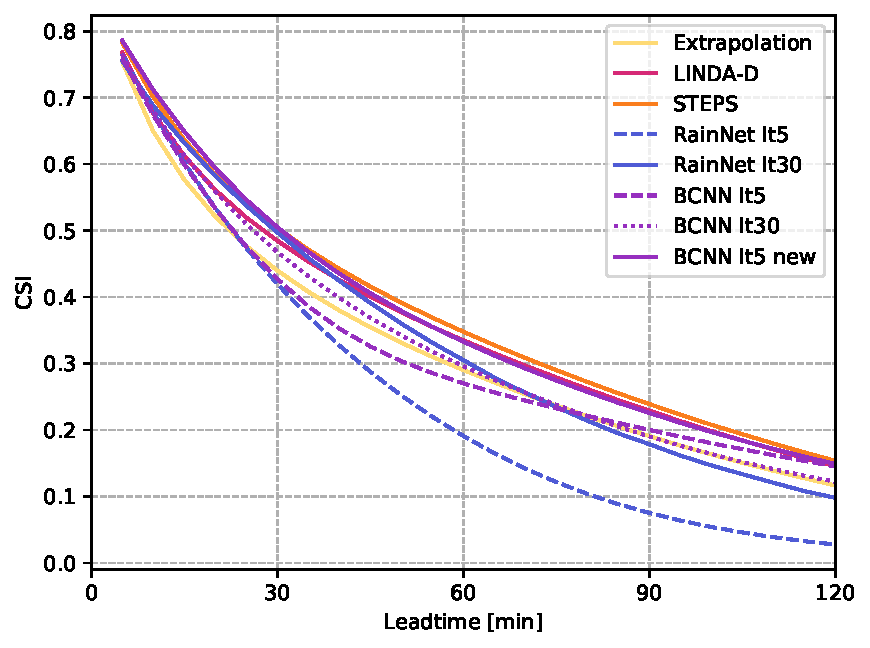
\includegraphics[width=0.33\textwidth]{images/metrics/ALL_CSI_0_5}}%
	\subfloat[5.0 mm/h]{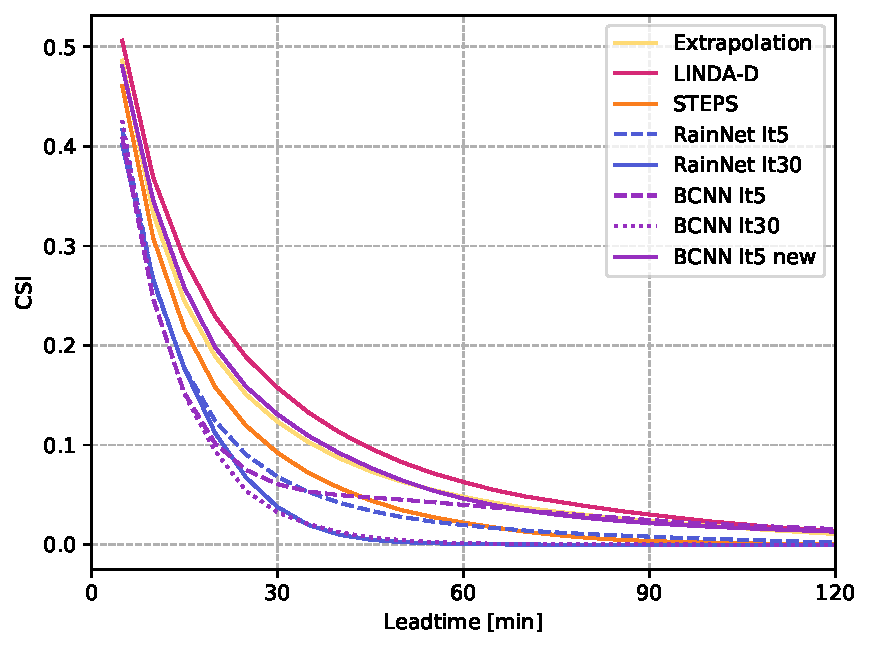
\includegraphics[width=0.33\textwidth]{images/metrics/ALL_CSI_5_0}}%
	\subfloat[20.0 mm/h]{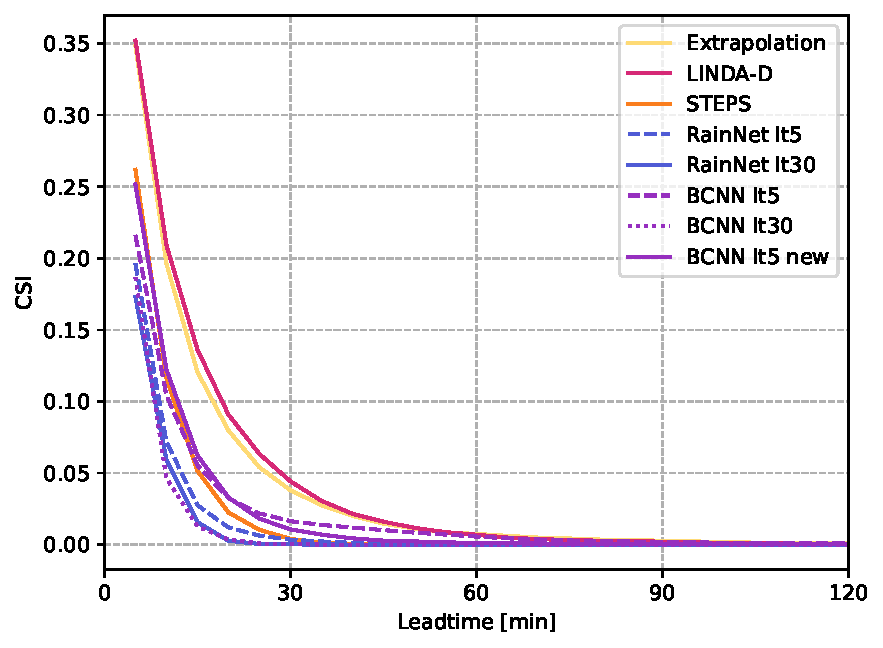
\includegraphics[width=0.33\textwidth]{images/metrics/ALL_CSI_20_0}}%
	\caption{CSI scores}
\end{figure}

\begin{figure}[ht]
	\label{fig:fss4}
	\subfloat[0.5 mm/h]{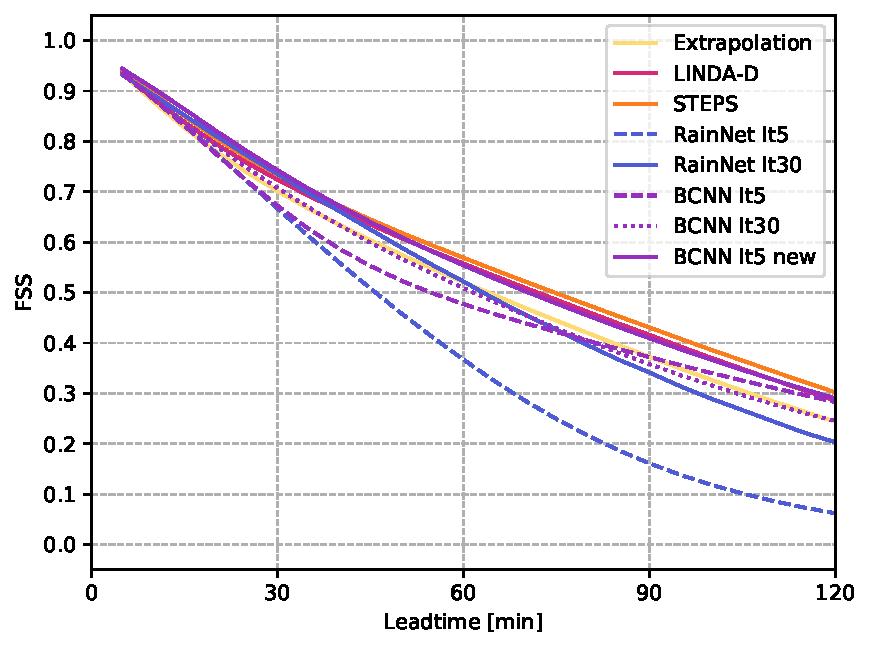
\includegraphics[width=0.33\textwidth]{images/metrics/ALL_FSS_2_0_5}}%
	\subfloat[5.0 mm/h]{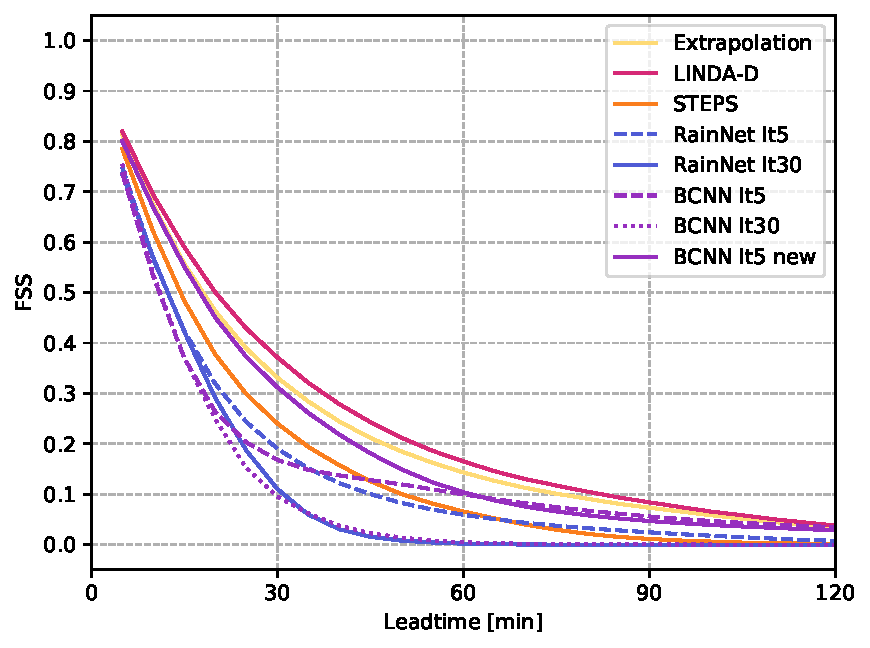
\includegraphics[width=0.33\textwidth]{images/metrics/ALL_FSS_2_5_0}}%
	\subfloat[20.0 mm/h]{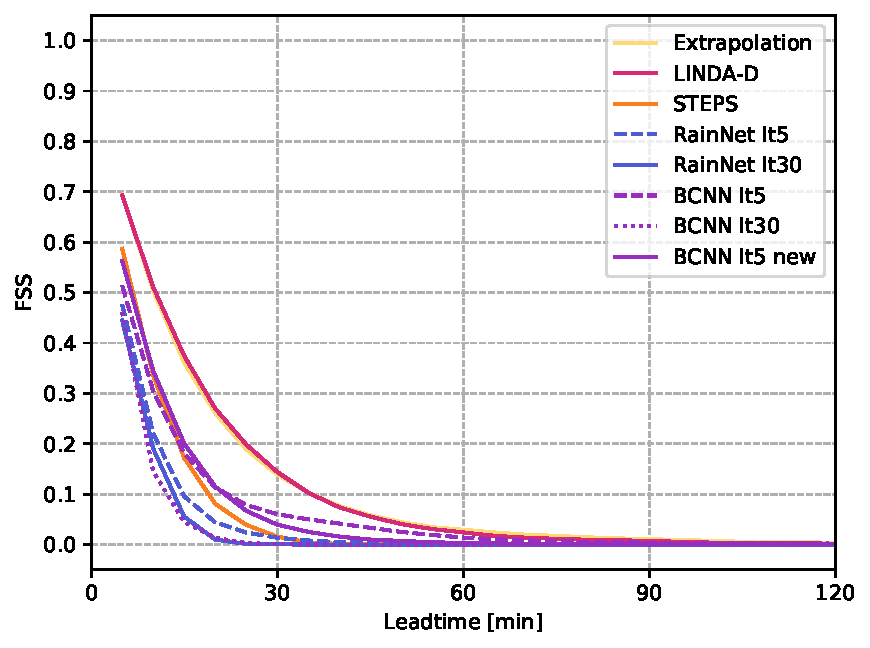
\includegraphics[width=0.33\textwidth]{images/metrics/ALL_FSS_2_20_0}}%
	\caption{FSS scores (4km)}
\end{figure}

\section{Probabilistic Metrics}




